\begin{figure}
	\floatbox{figure}[\FBwidth]
	{
		\caption{Calculating and interpreting readability scores}\label{figure2X}
	}
	{
	\begin{minipage}{0.7\textwidth}
		\small
		\begin{tabular}{ll}
			Score&Formula\\
			\midrule
			Flesch Reading Ease&$206.84-1.02\times\frac{\text{words}}{\text{sentences}}-84.60\times\frac{\text{syllables}}{\text{words}}$\\
			Flesch-Kincaid&$-15.59+0.39\times\frac{\text{words}}{\text{sentences}}+11.80\times\frac{\text{syllables}}{\text{words}}$\\
			Gunning Fog&$0.40\times\big(\frac{\text{words}}{\text{sentences}}+100\times\frac{\text{polysyllabic words}}{\text{words}}\big)$\\
			SMOG&$3.13+5.71\times\sqrt{\frac{\text{polysyllabic words}}{\text{sentences}}}$\\
			Dale-Chall&$3.64+0.05\times\frac{\text{words}}{\text{sentences}}+15.79\times\frac{\text{difficult words}}{\text{words}}$\\
		\end{tabular}
	\end{minipage}
	\begin{minipage}{0.25\textwidth}
		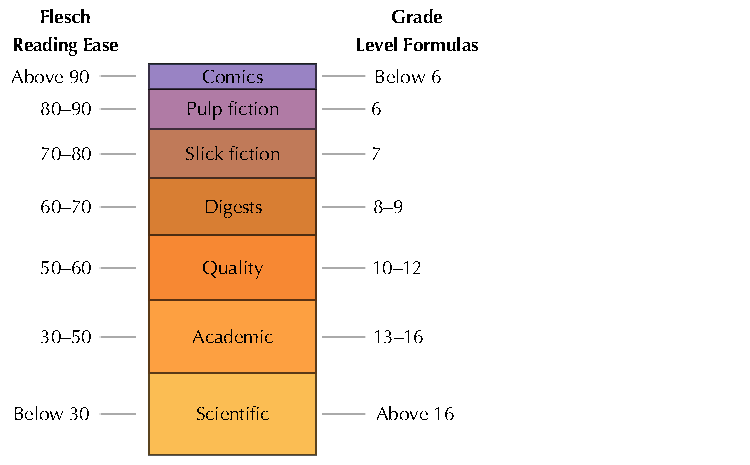
\includegraphics[trim=0cm 0cm 4.5cm 0cm, clip, width=\linewidth]{/Users/erinhengel/Dropbox/Readability/draft/pdf/therm.pdf}
	\end{minipage}
		\floatfoot{\tiny \textit{Notes}. Left-hand-side table displays the formula used to calculate each readability score. Polysyllabic words refers to words with three or more syllables; difficult words are those not found on a list of 3,000 words understood by 80 percent of fourth-grade readers (aged 9--10)~\citep{Chall1995}. The graphic on the right summarises the guidelines for interpreting different readability formulas~\citep{Flesch1962}.}
	}
\end{figure}